\subsection{Delay analysis}
\label{sec:analysis}

\subsubsection{Filtering irrelevant data}

Since the main focus of this thesis is to analyze the public transport network of Vienna, long-distance train services were stripped of the resulting data set. Since the \ac{API} endpoint does not differentiate between long-distance trains and suburban regional trains, the latter also were removed in this step. This means that in the following analysis, only public transport products by Wiener Linien, which includes metros, trams and buses, are considered. Long-distance trains have widely different characteristics in comparison to high-frequent inner-city transport methods such as trams or buses. These differences were quickly visible when conducting the first screening of the collected data. The most delayed trips were all Railjet (Austrian high-speed train service) services from neighboring countries, with delays in the multiple-hour range. While an interesting observation, these types of delays are not the intended research area of this thesis, which instead lays its focus on those inner city lines mentioned above. Additionally, the hybrid tram/train line \textit{Badner Bahn} also had to be excluded from further analysis since the collected data did only include scheduled timetable departures and not real-time departure times. This means that for this particular line, no delay data could be collected.

\subsubsection{Tools and technologies}

As mentioned in \cref{sec:persisting}, the resulting SQLite file was converted into a \ac{CSV} file for easier organization and handling. The following results were all gathered by utilizing the widely used data analysis library \textit{pandas} for Python. Visualizations on the resulting data frames were then produced by \textit{plotly}, another Python library commonly used for visualization and charting tasks. The most common figures such as line charts, bar charts, box plots or scatter plots are all available through the \textit{plotly-express} subpackage, which was used for all following visualizations. For figures including a map, the underlying map data is provided by \textit{Mapbox}.

\subsubsection{Basic summary}

To gather an initial overview of the collected data, we first want to highlight a few general characteristics of the data set. \Cref{table:basics} shows the basics statistical data points of the \texttt{delay} measurements. One can see that the mean delay was 14.68 seconds, with a minimum of -3600, meaning a one-hour early departure, and a maximum delay of 10,920 seconds, or approximately 3 hours. The high standard deviation of 115.62 seconds indicates that the data points are highly spread out around the mean. It is therefore unsurprising that the \nth{25}, \nth{50} and \nth{75} percentile are all 0 since actual punctuality rates of public transport networks mostly lay between 90 and 99 percent, for example with national rail services in Vienna having punctuality rates of around 96\% \autocite{oebb-2023b}. In fact, \cref{table:punctuality} shows that 12\% of the recorded departures had a delay greater than zero. However, the definition of punctuality varies from company to company and rates are usually calculated with a specified maximum delay threshold of one to five minutes \autocite[723]{chen-2009}. With a maximum delay of one minute, the punctuality rate falls at 94.17\%, while a maximum of five minutes results in 99.25\% punctuality. For all further punctuality rate calculations, we assume a departure is punctual if it has a maximum delay of three minutes or less.

\begin{table}
	\centering
	\begin{tabular}{lr}
		\toprule
		count &  13,720,398 \\
		mean  &  14.68 \\
		std   &  115.62 \\
		min   & -3600 \\
		25\%   &  0 \\
		50\%   &  0 \\
		75\%   &  0 \\
		max   &  10,920 \\
		\bottomrule
	\end{tabular}
	\caption{Basic summary of \texttt{delay} column}
	\label{table:basics}
\end{table}

\begin{table}
	\centering
	\begin{tabular}{rr}
		\toprule
		Delay threshold [min] & Punctuality rate \\
		\midrule
		0 &  0.8791 \\
		1  &  0.9417 \\
		2   &  0.9704 \\
		3   & 0.9837 \\
		4   & 0.9895 \\
		5   &  0.9925 \\
		\bottomrule
	\end{tabular}
	\caption{Punctuality rates depending on minimum delay}
	\label{table:punctuality}
\end{table}

\subsubsection{Most and least delayed lines}

When grouping all departures by line and sorting by punctuality rate, it shows that the most punctual lines are all bus lines, as shown in \cref{table:overall-top10-most}. Also, the nine most punctual lines all have perfect punctuality rates of 100\%, the first line with a rate less than 100\% is bus 54B with 99.98\%, landing in tenth place. Six of those lines with 100\% punctual departures even have a mean delay of 6 seconds or less, meaning only very few or no delays were recorded. Line N62 is the first one with a higher mean delay of 22.17 seconds, but still a perfect punctuality rate of 100\%. When looking at lines with the lowest punctuality rate in \cref{table:overall-top5-least}, one can see that again buses dominate and only one tram line appears as the fifth least punctual line, namely tram 71 with a punctuality rate of 95.51\% and a mean delay of 24.87 seconds. Line 42A has the lowest punctuality rate and also by far the highest mean delay with 149.01 seconds, while the other three bus lines show mean delays between 30.05 and 51.89 seconds.

\begin{table}
	\centering
	\begin{tabular}{llrr}
		\toprule
		Line & Product & Punctuality rate & Mean delay [s] \\
		\midrule
		ZF & Bus &  1.0 & 0.00 \\
		73A & Bus &  1.0 & 0.00 \\
		34A & Bus &  1.0 & 0.00 \\
		U6E & Metro/bus &  1.0 & 0.00 \\
		N29 & Bus &  1.0 & 0.97 \\
		N66 & Bus &  1.0 & 1.54 \\
		2A & Bus & 1.0 & 1.69 \\
		N46 & Bus &  1.0 & 5.99 \\
		N62 & Bus & 1.0 & 22.17 \\
		54B & Bus &  0.9998 & 4.56 \\
		\bottomrule
	\end{tabular}
	\caption{Top ten most punctual lines}
	\label{table:overall-top10-most}
\end{table}

\begin{table}
	\centering
	\begin{tabular}{llrr}
		\toprule
		Line & Product & Punctuality rate & Mean delay [s] \\
		\midrule
		42A & Bus & 0.9030 & 149.01 \\
		10A & Bus &  0.9245 & 51.89 \\
		63A & Bus &  0.9505 & 30.05 \\
		95A & Bus & 0.9527 & 39.14 \\
		71 & Tram &  0.9551 & 24.87 \\
		\bottomrule
	\end{tabular}
	\caption{Top five least punctual lines}
	\label{table:overall-top5-least}
\end{table}

Because of the dominance of bus lines, a further differentiation between bus, tram and metro lines may be of interest. \Cref{table:metro-top5} shows the city's five metro lines ordered by their punctuality rate. Line U6E is a special case as it is categorized as a metro line while it actually operated as a bus and acted as a replacement for a few stops on line U6 during one weekend of construction work. All other, actual metro lines show quite high punctuality rates too, with U2 being the least punctual line which still had 98.65\% punctual departures. Line U6 is the most punctual line, showing a punctuality rate of 99.5\%. Mean delays generally increase for lower punctuality rates, though remain at a low level with values between 7.89 and 18.52 seconds.

\begin{table}
	\centering
	\begin{tabular}{lrr}
		\toprule
		Line & Punctuality rate & Mean delay [s] \\
		\midrule
		U6E & 1.0 & 0.00 \\
		U6 &   0.9950 & 10.14 \\
		U1 &   0.9944 & 7.89 \\
		U3 &   0.9926 & 12.11 \\
		U4 &   0.9882 & 14.95 \\
		U2 &   0.9865 & 18.52 \\
		\bottomrule
	\end{tabular}
	\caption{Metro lines by punctuality rate}
	\label{table:metro-top5}
\end{table}

\Cref{table:tram-top5-most} and \cref{table:tram-top5-least} show only tram lines, with line 52 showing the highest punctuality rate of 99.77\% and line 71 the lowest with 95.51\%. Similar to U6E, U2Z is a replacement line during construction work. However, in daily operation, it is treated like a regular tram line, as it is planned to be in service for more than two years \autocite{stadt-wien-2021}. For the most punctual trams, mean delays show very low values, with three out of the top five having negative values ranging as low as -32.24 seconds for line U2Z. The least punctual trams lines have mean delays of around 30 seconds, only line 1 has a lower value of 10.88 seconds.


\begin{table}
	\centering
	\begin{tabular}{lrr}
		\toprule
		Line & Punctuality rate & Mean delay [s] \\
		\midrule
		52 &  0.9977 & 4.22 \\
		U2Z &  0.9955 & -32.24 \\
		33 &   0.9954 & -15.99 \\
		37 &   0.9929 & 10.53 \\
		30 &   0.9928 & -2.41 \\
		\bottomrule
	\end{tabular}
	\caption{Top five most punctual tram lines}
	\label{table:tram-top5-most}
\end{table}

\begin{table}
	\centering
	\begin{tabular}{lrr}
		\toprule
		Line & Punctuality rate & Mean delay [s] \\
		\midrule
		71 &  0.9551 & 24.87 \\
		2 &   0.9554 & 26.62 \\
		1 &   0.9678 & 10.88 \\
		D &   0.9727 & 32.49 \\
		O &   0.9737 & 23.80 \\
		\bottomrule
	\end{tabular}
	\caption{Top five least punctual tram lines}
	\label{table:tram-top5-least}
\end{table}

\subsubsection{Most and least delayed stations}

Following the fact that entire lines showed punctuality rates of 100\%, all stations that serve these lines (but not others), also have a punctuality rate of 100\%. More interesting are the stations with the lowest rates of punctual departures, shown in \cref{table:stations-least-10}. They are all bus stops again, interestingly however the very least punctual stop, \textit{Blaasstraße}, has a difference in punctuality rate to the next one (i.e. second least punctual) of almost eight percentage points while the maximum difference of all other neighboring punctuality rates in fact lies at 0.87 percentage points. Also, while mean delay values are generally high for the least punctual stations, they do not strictly increase with lower punctuality rates. \textit{Krenngasse}, for example, has the fifth-highest mean delay but ranks tenth for punctuality rate. \Cref{fig:boxplot-stations} shows box plots of the stations' delays with stations grouped by their available products. In these plots, \textit{Blaasstraße} is clearly visible on the very left of the plot for bus stations and overall, indicating it is an outlier.

Again, since most and least delayed stations are all bus stations and to get more results about highly frequented stations that are relevant to more passengers, \cref{table:metro-stations-top5-most} shows only the highest-ranked stations that serve at least one metro line, while \cref{table:metro-stations-top5-least} shows the five least punctual metro stations in the network. Of those stations, \textit{Neue Donau} is the most punctual with a punctuality rate of 99.9\%, while \textit{Aspern Nord} shows the most delays with its punctuality rate being 97.11\%. The five most punctual stations show low mean delays between 2.73 and 10.71 seconds while the least punctual metro stations still have mean delays of around 20 seconds, only five seconds higher than the average of the whole data set. Three out of the five stations with the lowest punctuality rates serve metro, tram and bus lines, while all of the five most punctual stations have metro and bus services only.

\begin{figure}[h]
	\centering
	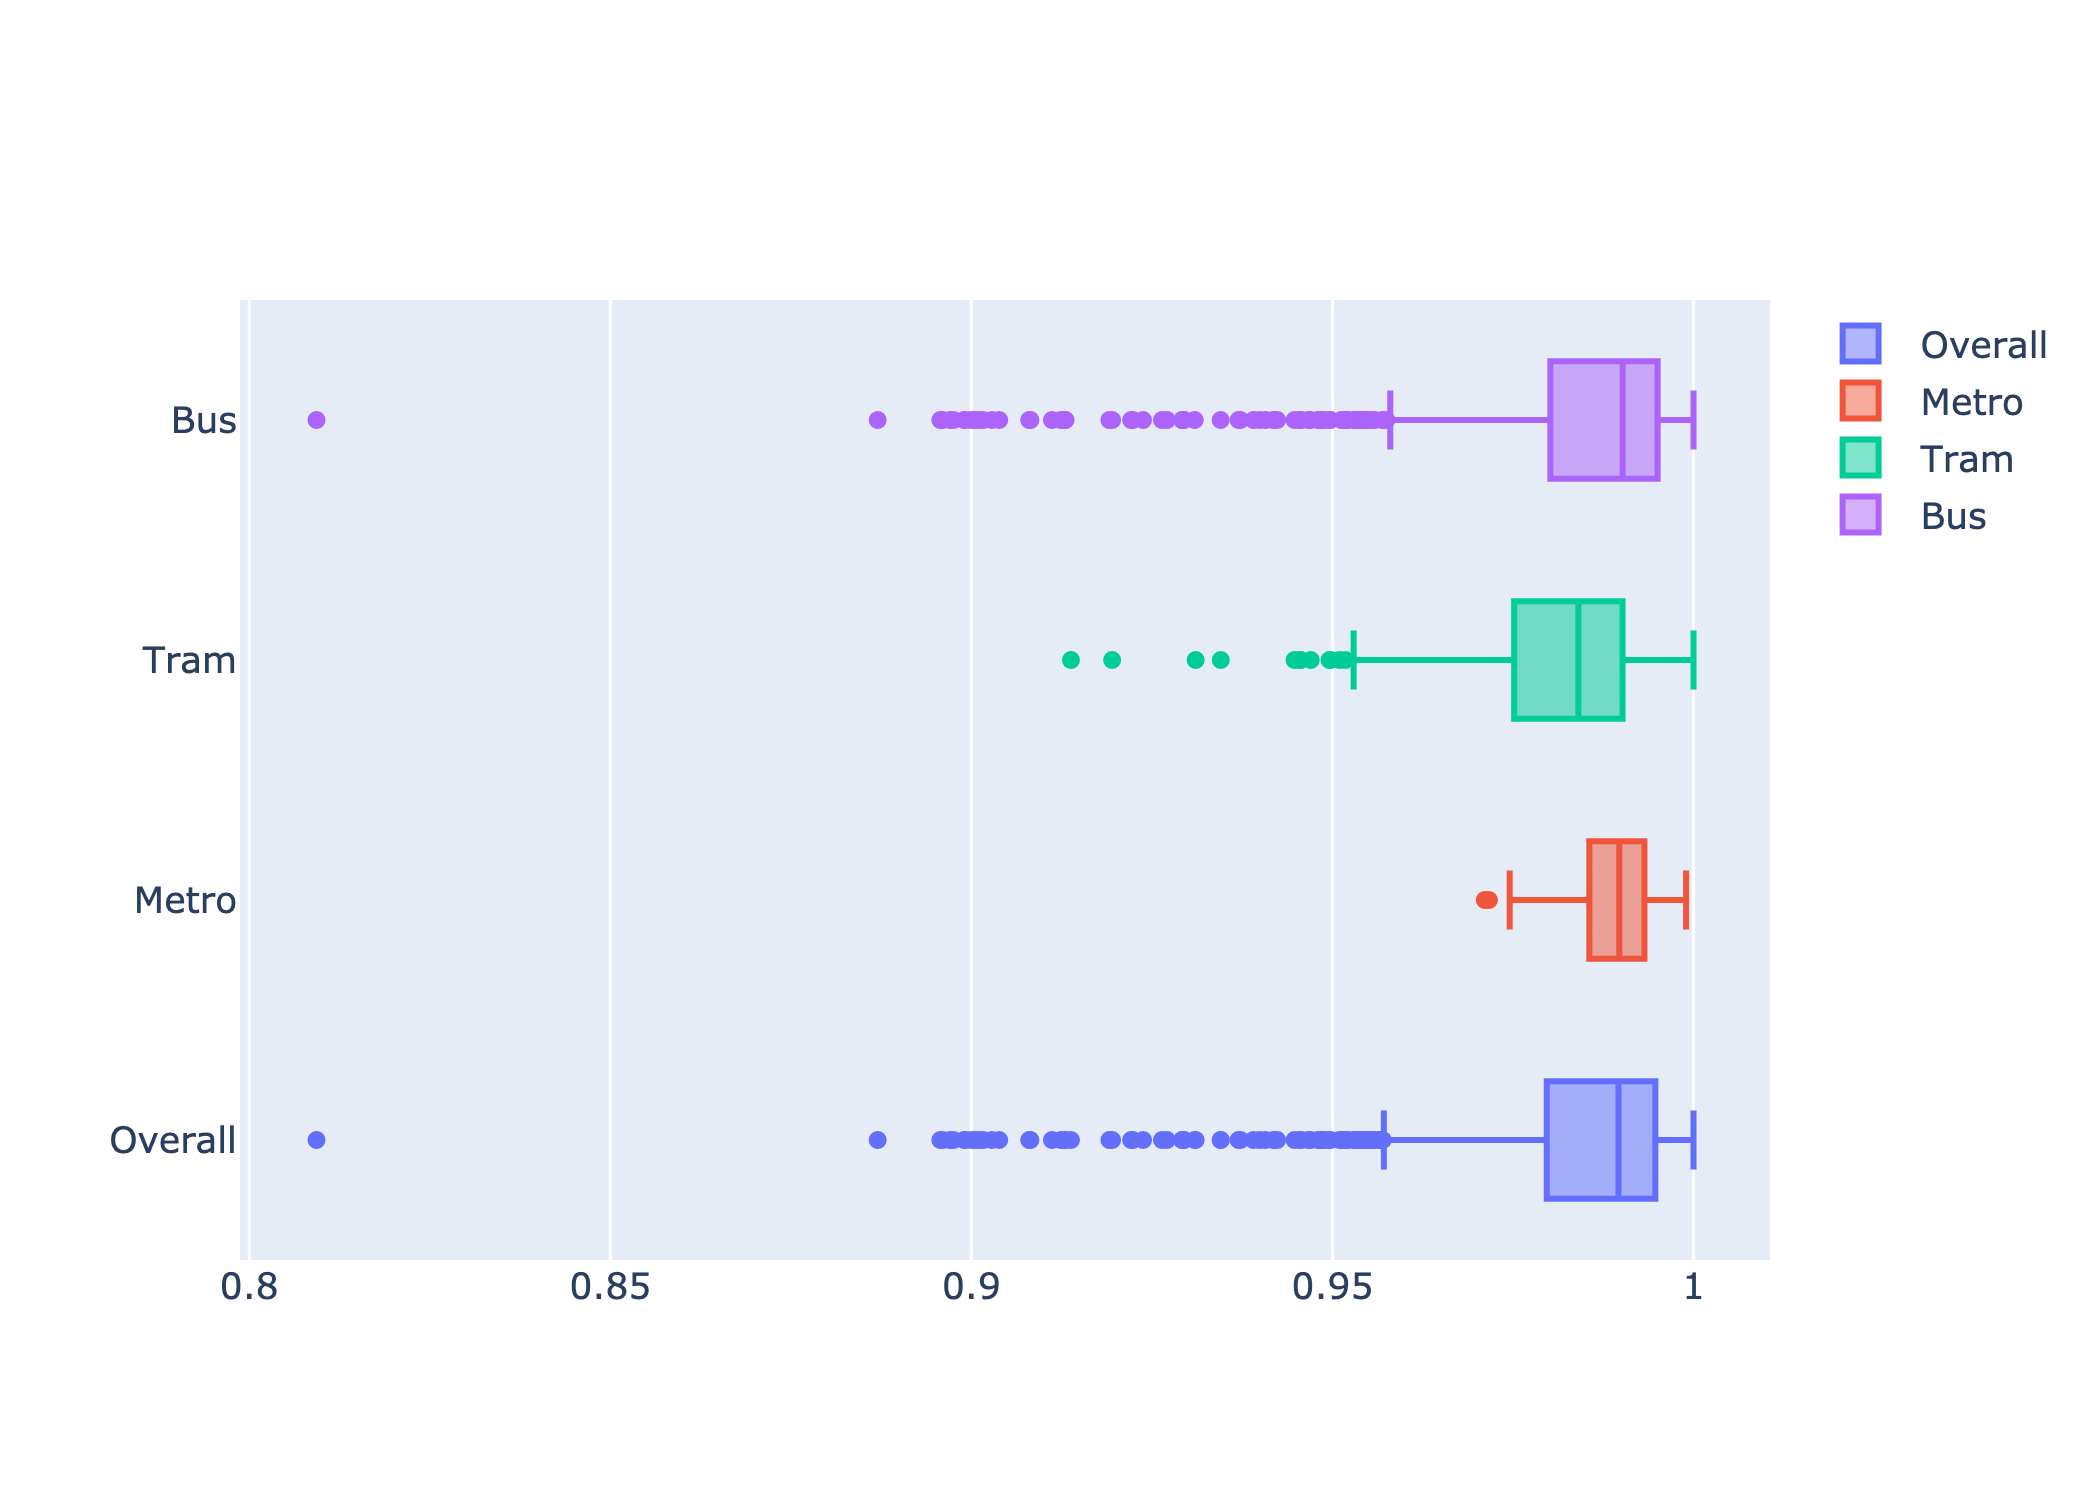
\includegraphics[width=0.9\textwidth]{boxplot-stations}
	\caption{Box plots of delay rates grouped by station type}
	\label{fig:boxplot-stations}
\end{figure}

\begin{table}
	\centering
	\begin{tabular}{llrr}
		\toprule
		Station & Products & Punctuality rate & Mean delay [s] \\
		\midrule
		Blaasstraße & Bus & 0.8093 & 115.53 \\
		Schafbergbad & Bus &  0.8870 & 178.62 \\
		Schafberg/Werfelstraße & Bus &  0.8957 & 164.45 \\
		Twarochgasse & Bus &   0.8961 & 164.66 \\
		Minciostraße & Bus &   0.8971 & 83.30 \\
		Ulanenweg & Bus &   0.8975 & 62.63 \\
		Kieslerweg & Bus &   0.8990 & 67.12 \\
		KGV Alsrückenweg & Bus &   0.8991 & 155.32 \\
		Korbweidenweg & Bus &   0.9000 & 70.19 \\
		Krenngasse & Bus &   0.9005 & 153.04 \\
		\bottomrule
	\end{tabular}
	\caption{Top ten least punctual stations}
	\label{table:stations-least-10}
\end{table}


\begin{table}
	\centering
	\begin{tabular}{llrr}
		\toprule
		Station & Products & Punctuality rate & Mean delay [s] \\
		\midrule
		Neue Donau & Metro, bus & 0.9990 & 2.73 \\
		Siebenhirten & Metro, bus &  0.9988 & 5.17 \\
		Hütteldorf & Metro, bus  & 0.9987 & 3.47 \\
		Seestadt & Metro, bus & 0.9984 & 10.71 \\
		Nestroyplatz &  Metro, bus  & 0.9966 & 6.28 \\
		\bottomrule
	\end{tabular}
	\caption{Top five most punctual stations serving metro lines}
	\label{table:metro-stations-top5-most}
\end{table}

\begin{table}
	\centering
	\begin{tabular}{llrr}
		\toprule
		Station & Products & Punctuality rate & Mean delay [s] \\
		\midrule
		Aspern Nord & Metro, bus & 0.9711 & 21.36 \\
		Taborstraße & Metro, tram, bus &  0.9717 & 21.40\\
		Johnstraße & Metro, tram, bus & 0.9746 & 23.66 \\
		Meidling Hauptstraße & Metro, bus & 0.9785 & 17.75 \\
		Schwedenplatz &  Metro, tram, bus & 0.9789 & 15.21 \\
		\bottomrule
	\end{tabular}
	\caption{Top five least punctual stations serving metro lines}
	\label{table:metro-stations-top5-least}
\end{table}

\subsubsection{Tram line 71}
\label{sec:line-71-analysis}

In previous sections, all lines or stations of the network were considered. In this section, we want to analyze and focus on one specific line. For this, tram line 71 was chosen for three reasons: Firstly, it is a highly frequented line with intervals of 7-8 minutes on weekdays and therefore much departure data was collected and is available for analysis. Secondly, it is a radial line, starting in the city center and terminating in an outer district. This type of line represents the majority of tram lines in the network. Finally, it is the tram line with the lowest punctuality rate, promising interesting results for delay measures along the line. 

\Cref{table:tram-71-stations} shows all 32 stations on line 71 sorted by their respective punctuality rate. Additionally, the mean delay was calculated for each station. The most punctual station is \textit{Kasierebersdorf, Zinnergasse} which shows a punctuality rate of 99.59\% and a mean delay of -25.15 seconds. All other stations have positive mean delays with values ranging between 18.35 and 33.63 seconds. The least punctual station, \textit{Valiergasse}, has a punctuality rate of 92.30\% and said mean delay of 33.63 seconds. Additionally, one can see that the mean delay generally increases with a lower ranking and thus lower punctuality rate. However, certain stations do not follow this pattern and show a higher mean delay than the next station down the list. For example, \textit{Ring/Volkstheater U} has with 20.42 seconds a notably higher mean delay value than the next less punctual station, \textit{Am Heumarkt}, which has a mean delay of 18.71 seconds. The same behavior can be observed for \textit{Oper/Karlsplatz U} and its neighbor in the table \textit{Unteres Belvedere}.

\begin{table}
	\centering
	\begin{tabular}{lrr}
		\toprule
		Station & Punctuality rate & Mean delay [s] \\
		\midrule
		Kaiserebersdorf, Zinnergasse &    0.9959 & -25.15 \\
		Rathausplatz/Burgtheater     &    0.9796 &  18.35 \\
		Parlament                    &    0.9788 &  18.48 \\
		Burgring                     &    0.9785 &  19.35 \\
		Börse                        &    0.9784 &  18.83 \\
		Ring/Volkstheater U          &    0.9769 &  20.42 \\
		Am Heumarkt                  &    0.9757 &  18.71 \\
		Schottentor                  &    0.9747 &  22.08 \\
		Schwarzenbergplatz           &    0.9736 &  20.88 \\
		Oper/Karlsplatz U            &    0.9734 &  23.77 \\
		Unteres Belvedere            &    0.9699 &  21.18 \\
		Rennweg                      &    0.9697 &  22.10 \\
		Kleistgasse                  &    0.9679 &  20.34 \\
		Oberzellergasse              &    0.9666 &  20.40 \\
		St. Marx                     &    0.9654 &  22.72 \\
		Litfaßstraße                 &    0.9566 &  25.04 \\
		Molitorgasse                 &    0.9554 &  25.76 \\
		Zippererstraße               &    0.9545 &  25.12 \\
		Hauffgasse                   &    0.9526 &  26.26 \\
		Enkplatz                     &    0.9459 &  29.50 \\
		Simmering                    &    0.9444 &  30.23 \\
		Braunhubergasse              &    0.9441 &  29.26 \\
		Fickeysstraße                &    0.9424 &  29.95 \\
		Weißenböckstraße             &    0.9414 &  29.48 \\
		Zentralfriedhof 1.Tor        &    0.9393 &  29.49 \\
		Zentralfriedhof 2.Tor        &    0.9369 &  30.57 \\
		Zentralfriedhof 3.Tor        &    0.9337 &  31.50 \\
		Pantucekgasse/Widholzgasse   &    0.9334 &  30.75 \\
		Zentralfriedhof 4.Tor        &    0.9329 &  30.89 \\
		Leberberg                    &    0.9322 &  30.87 \\
		Svetelskystraße              &    0.9288 &  31.78 \\
		Valiergasse                  &    0.9230 &  33.63 \\
		\bottomrule
	\end{tabular}
	\caption{Stations on line 71 sorted by punctuality rate}
	\label{table:tram-71-stations}
\end{table}

\subsubsection{Station \textit{Karlsplatz}}

\begin{table}
	\centering
	\begin{tabular}{llrr}
		\toprule
		Line & Product & Punctuality rate & Mean delay [s] \\
		\midrule
		2A & Bus & 0.9970 & 3.75 \\
		U2Z & Tram & 0.9965 & -16.20 \\
		U1 & Metro & 0.9948 & 8.29 \\
		4A & Bus & 0.9889 & 12.69 \\
		59A & Bus & 0.9854 & 18.83 \\
		U4 & Metro & 0.9811 & 17.84 \\
		71 & Tram & 0.9734 & 23.77 \\
		1 & Tram & 0.9724 & 0.76 \\
		D & Tram & 0.9721 & 37.09 \\
		62 & Tram & 0.9702 & 30.18 \\
		2 & Tram & 0.9567 & 29.59 \\
		\bottomrule
	\end{tabular}
	\caption{Lines at \textit{Karlsplatz} sorted by punctuality rate}
	\label{table:karlsplatz-lines}
\end{table}

Like \cref{sec:line-71-analysis} did for one line, this section focuses on the analysis of one station. For this, the station \textit{Karlsplatz} was chosen, as it is one of the main transfer hubs in the network. It serves two metro lines, six tram lines and three bus lines. When construction finishes in the fall of 2023, the station's third metro line U2 will continue its service to \textit{Karlsplatz}. In the meantime, tram U2Z serves as a replacement line, with one of its terminal stations located at \textit{Karlsplatz}.

In \cref{table:karlsplatz-lines}, departures at \textit{Karlsplatz} are grouped by lines and again sorted by their respective punctuality rate. Line 2A, one of the inner city buses has the best punctuality rate with 99.70\% punctual departures, together with a mean delay of 3.75 seconds. Next is U2Z, the replacement tram line for U2, showing a punctuality rate of 99.65\% and, notably, a mean delay of -16.20 seconds. Metro lines U1 and U4 show considerably lower mean delays than tram lines, with U1 having a rather low value of just 8.29 seconds and a punctuality rate of 99.48\%. Interestingly, tram lines 71, D, 62 and 2 all have similar mean delays of approximately 30 seconds. Line 1 however has a mean delay of only 0.76 seconds, even though its punctuality rate of 97.24\% is similar to the other mentioned lines. The line with the least number of punctual departures is tram line 2 with its punctuality rate of 95.67\% and mean delay of 29.59 seconds.